\chapter{Couple Mode Theory}
\label{chap:couple_mode}
%Descrição dos modos a1 e a3 considerando a perturbação de terceira ordem no autovalor. No final da sessão vou ter descrito a teoria do mapa de eficiência. Aqui uso como gancho a necessidade de saber os valores de $\kappa_e$ e $\kappa_i$ do visível e o valor de $J_3$ como motivação para todo o resto.  

The cavities we fabricate are designed to presents multiples optical modes. In this Chapter we shall study how the nonlinearity of the material affect this modes. Initially a infrared mode are excited using a external source, the third harmonic of the source act as a new source with the triple of the frequency in the neighborhood of a visible mode, leading to a couple behavior of this modes, this coupling can be described using the rate equation  

\section{Couple Rate Equation}
%
%From now on we are interested in optical mode with specific feature. Let's assume a mode with frequency $\omega_1$ at infrared, we want to know how it couple with a visible mode of frequency $\omega_3 = 3\times\omega_1+\delta$. 
%
%\begin{subequations}
%    \begin{alignat}{2}
%        \dot{a}_1 &= -\left(i\Delta_1 + i\omega_1 A_1|a_1|^2 + i\omega_1 A_{13}|a_3|^2 + \frac{\kappa_1}{2}\right)a_1 + \sqrt{\kappa^{(e)}_1}S_{in},\\
%        \dot{a}_3 &= -\left(i\Delta_3 + i\omega_3 A_3|a_3|^2+ i\omega_3 A_{31}|a_1|^2 + \frac{\kappa_3}{2}\right)a_3.
%    \end{alignat}
%\end{subequations}

The Eq~\ref{eq:rate_equation_bistable} give us the behavior of a single mode. For problems with low nonlinearity, when is possible to neglect terms of order $\left(\chi^{(n)}\right)^2$ and highers, the effect of the nonlinearity can be found using perturbation theory. 
\begin{equation}
    \frac{\delta\omega_\alpha}{\omega_\alpha} = \frac{1}{2}\frac{\bra{\vec{E}_\alpha}\delta\epsilon\ket{\vec{E}}}{\braket{\vec{E}_\alpha|\vec{E}_\alpha}} = \frac{1}{2}\frac{\int\vec{E}^*_\alpha\delta\vec{P}d^3\vec{r}}{\int \epsilon|\vec{E}_\alpha|^2d^3\vec{r}}
    \label{eq:perp_theory}
\end{equation}
Note that $\vec{E}_\alpha$ is the unperturbed electric field of the $\alpha$th mode, while $\vec{E}$ is the total electric field. 

For a generic problem $\delta\epsilon\ket{\vec{E}}=\ket{\delta\vec{P}}$ is the change in the polarization due to nonlinearity perturbation, as we are studding third order nonlinearity this perturbation can be write as $\delta\vec{P} = \epsilon\chi^{(3)}|\vec{E}|^2\vec{E}$. Our model assumes that there is only two different modes coupled, in such way that the total electric field is
\begin{equation}
    \vec{E} = \vec{E}_1+\vec{E}_3+c.c.
\end{equation}
From now on, the label $1$ refers to the model in the infrared and the label $3$ to the mode in the visible. 
The calculus of the Eq~\ref{eq:perp_theory} give rise to a total of sixty four terms for each one of the modes; however, most of then are not of our interest. In order to filter this terms we will write the electric field with a explicit dependency of time $\vec{E}_\alpha(\vec{r},t) = a_\alpha(t) \vec{e}_\alpha(\vec{r})$. Considering the approximation of slowly variation, the amplitude $a_\alpha(t)$ can be considered as a harmonic function with frequency $\omega_\alpha$. Applying this trick, some terms of the Eq~\ref{eq:perp_theory} can be considered out of frequency and be neglected. The full expression for the perturbation for each mode is

\begin{eqnarray}
\frac{\delta\omega_1}{\omega_1} &=& -\frac{1}{8}\left[|a_1|^2\frac{\int\epsilon\chi^{(3)}
\Big(|\vec{e}_1\cdot\vec{e}_1|^2 + 2|\vec{e}_1\cdot\vec{e}_1^*|^2
\Big)d^3\vec{r}}
{\int \epsilon|\vec{e}_1|^2 d^3\vec{r}}\right. +\nonumber\\
&+&2|a_3|^2\frac{\int\epsilon\chi^{(3)}
\Big((\vec{e}_1\cdot\vec{e}_1^*)(\vec{e}_3\cdot\vec{e}_3^*)+|\vec{e}_1\cdot\vec{e}_3|^2+|\vec{e}_1\cdot\vec{e}^*_3|^2
\Big)d^3\vec{r}}
{\int \epsilon|\vec{e}_1|^2 d^3\vec{r}}+\nonumber\\
&+&\left.\frac{(a^*_1)^2a_3}{a_1}\frac{\int\epsilon\chi^{(3)}
\Big(3(\vec{e}^*_1\cdot\vec{e}_1^*)(\vec{e}^*_1\cdot\vec{e}_3)
\Big)d^3\vec{r}}
{\int \epsilon|\vec{e}_1|^2 d^3\vec{r}}\right]
\end{eqnarray}

\begin{eqnarray}
\frac{\delta\omega_3}{\omega_3} &=& -\frac{1}{8}\left[|a_3|^2\frac{\int\epsilon\chi^{(3)}
\Big(|\vec{e}_3\cdot\vec{e}_3|^2 + 2|\vec{e}_3\cdot\vec{e}_3^*|^2
\Big)d^3\vec{r}}
{\int \epsilon|\vec{e}_3|^2 d^3\vec{r}}\right. +\nonumber\\
&+&2|a_1|^2\frac{\int\epsilon\chi^{(3)}
\Big((\vec{e}_1\cdot\vec{e}_1^*)(\vec{e}_3\cdot\vec{e}_3^*)+|\vec{e}_1\cdot\vec{e}_3|^2+|\vec{e}_1\cdot\vec{e}^*_3|^2
\Big)d^3\vec{r}}
{\int \epsilon|\vec{e}_3|^2 d^3\vec{r}}+\nonumber\\
&+&\left.\frac{(a_1)^3}{a_3}\frac{\int\epsilon\chi^{(3)}
\Big(3(\vec{e}_1\cdot\vec{e}_1)(\vec{e}_1\cdot\vec{e}^*_3)
\Big)d^3\vec{r}}
{\int \epsilon|\vec{e}_3|^2 d^3\vec{r}}\right]
\end{eqnarray}

In order to normalize the amplitude in such way that $|a_\alpha(t)|^2$ is the energy stored in the $\alpha$th mode, we should normalize the electric field $\vec{e}_\alpha \rightarrow\vec{e}_\alpha/\int|\vec{e}_\alpha|^2 d^3\vec{r}$. Using this form, the perturbation can be linked with the rate equation making $\omega_\alpha \rightarrow \omega_\alpha + \delta\omega_\alpha$. We can factorize the expression based in the dependence of the amplitude. 

\begin{eqnarray}
\frac{\delta\omega_1}{\omega_1} &=& A_{11}|a_1|^2 + A_{13}|a_3|^2 + B_1\frac{(a^*_1)^2a_3}{a_1},\label{eq:ir_per}\\
\frac{\delta\omega_3}{\omega_3} &=& A_{33}|a_3|^2 + A_{31}|a_1|^2 + B_3\frac{(a_1)^3}{a_3}\label{eq:vis_per}.
\end{eqnarray}

%The rate equation for both modes are write as
Once identified all terms, we use the rotation frame approximation making $a_1 \rightarrow a_1e^{i\omega t}$ and $a_3 \rightarrow a_3e^{i3\omega t}$, with $\omega$ being the source frequency. Them we have 
\begin{subequations}
    \begin{alignat}{1}
        \dot{a}_1 &= -\left(i\Delta_1 + \omega_1i(A_{11} |a_1|^2 + A_{13} |a_3|^2) + \kappa_{1}\right)a_1 - i\omega_1 B_1(a^*_1)^2a_3 
        +\sqrt{2 \kappa^{(e)}_1}S_{in}
        \label{eq:taxa_ir_broad}\\
        \dot{a}_3 &= -\left(i\Delta_3 + \omega_3i(A_{31} |a_1|^2 + A_{33} |a_3|^2) + \kappa_{3}\right)a_3 - i\omega_3 B_3(a_1)^3.
        \label{eq:taxa_vis_broad}
    \end{alignat}
    \label{eq:rate_broad}
\end{subequations}
This move lead us to few new terms. Let's take a look to each one of them. First, we define $\Delta_1 = \omega_1 - \omega$ and $\Delta_3 = \omega_3 - 3\times\omega$. 

The terms $A_{\alpha\alpha}$ look like to the SPM term presented in Eq~\ref{eq:rate_equation_bistable}, in fact both are responsible for the same effect. 

The directly dependence of the refractive index with the intensity of the electric field is called the Optical Kerr effect. It is possible to show that due to third order nonlinearity, the refractive index can be write as~\needcit
\begin{equation}
    \text{n} = \text{n}_0 + 2\bar{\text{n}}_2|E|^2 
\end{equation}
If included in the wave equation, it lead to the same bistable behavior discussed before. The difference between Kerr bistability and thermotic bistability lies in the nature of both. The Kerr effect responds at a time scale faster than thermotic\needcit~ and have to due just with the material, meanwhile the thermotic bistability is a intrinsic behavior of the optical cavity and can be affect by both, material and geometry. However, at the specific experimental condition, we can not distinguish the individual contribution of each one in the transmission~\needcit, hence we consider just one SPM term that includes contributions of both, Kerr and thermotic. 

Futhermore, the Eqs~\ref{eq:rate_broad} present another similar term, with the form $A_{ij}|a_j|^2$. The effec of this term is exactly the one discussed before, but the bistability are generated due to the other optical mode, for both Kerr and thermotic~\needcit. This term are called Cross Phase Modulation (XPM). The expression for Kerr SPM and XPM can be take from the perturbation theory as 


\begin{subequations}
    \begin{alignat}{1}
        A_{ii} &= \frac{1}{8}\frac{\int\epsilon\chi^{(3)}
        \Big[|\vec{e}_i\cdot\vec{e}_i|^2 + 2|\vec{e}_i\cdot\vec{e}_i^*|^2
        \Big]d^3\vec{r}}{\Big[\int \epsilon|\vec{e}_i|^2 d^3\vec{r}\Big]^2},
        \\
        A_{ji} &= \frac{1}{4}\frac{\int\epsilon\chi^{(3)}
        \Big[|\vec{e}_i|^2|\vec{e}_j|^2 + |\vec{e}_i\cdot\vec{e}_j|^2+ |\vec{e}_i\cdot\vec{e}_j^*|^2
        \Big]d^3\vec{r}}{\Big[\int \epsilon|\vec{e}_i|^2 d^3\vec{r}\Big]\Big[\int \epsilon|\vec{e}_j|^2 d^3\vec{r}\Big]}.
    \end{alignat}
\end{subequations}

The other new terms are $B_1$ and $B_3$.% It is important to emphasize the fact that the amplitude $a_\omega$ is complex, so this term presents a real and a imaginary part, which act as a source term. 
We will call it the Coupling term, it is responsible for convert energy from one mode to the other. The expression for both, can be take from the perturbation theory as
\begin{subequations}
    \begin{alignat}{1}
        B_{1} &= \frac{3}{8}\frac{\int\epsilon\chi^{(3)}
        (\vec{e}_1^*\cdot\vec{e}_1^*)(\vec{e}_1^*\cdot\vec{e}_3)
        d^3\vec{r}}{\Big[\int \epsilon|\vec{e}_1|^2 d^3\vec{r}\Big]^{3/2}\Big[\int \epsilon|\vec{e}_3|^2 d^3\vec{r}\Big]^{1/2}},
        \label{eq:coupling_b1}
        \\
        B_{3} &= \frac{1}{8}\frac{\int\epsilon\chi^{(3)}
        (\vec{e}_1\cdot\vec{e}_1)(\vec{e}_1\cdot\vec{e}^*_3)
        d^3\vec{r}}{\Big[\int \epsilon|\vec{e}_1|^2 d^3\vec{r}\Big]^{3/2}\Big[\int \epsilon|\vec{e}_3|^2 d^3\vec{r}\Big]^{1/2}}.
        \label{eq:coupling_b3}
    \end{alignat}
    \label{eq:coupling}
\end{subequations}

%Using energy conservation $\frac{d}{dt}\left(|a_1|^2+|a_3|^2\right) = 0$ we can find that $\omega_1B_1 = \omega_3B^*_3$ 
In order to solve the Coupled Rate Equations Eq~\ref{eq:rate_broad} we will use a numerical method with the software Mathematica, the Appendix~\ref{app:numerical_met} treat about the method, now we are interested in the results. 

\section{Coupling Coefficient}

The first interesting result come from the coefficients $B_1$ and $B_3$, it told us how a infrared photon is scattered for the visible modes. The spatial dependence of the electric field is important as the coupling coefficient depends on the overlap integral between the modes defined as 
\begin{eqnarray}
J_3 = \frac{\int
        (\vec{e}_1\cdot\vec{e}_1)(\vec{e}_1\cdot\vec{e}^*_3)
        d^3\vec{r}}{\Big[\int \epsilon|\vec{e}_1|^2 d^3\vec{r}\Big]^{3/2}\Big[\int \epsilon|\vec{e}_3|^2 d^3\vec{r}\Big]^{1/2}}
\end{eqnarray}

Before to simulate the modes to calculate the overlap integral let's consider the symmetry of the problem. The WGM presents a harmonic dependence in the azimuthal coordinate, thus enable us to write the electric field as $\vec{e_\alpha}(\vec{r}) = \vec{e_\alpha}(r,z)e^{-im_\alpha\theta}+c.c.$ which lead to a overlap integral with the form
\begin{equation}
    J_3 = \frac{\iint
        (\vec{e}_1(r,z)\cdot\vec{e}_1(r,z))(\vec{e}_1(r,z)\cdot\vec{e}^*_3(r,z))
        drdz}{\Big[\int \epsilon|\vec{e}_1|^2 d^3\vec{r}\Big]^{3/2}\Big[\int \epsilon|\vec{e}_3|^2 d^3\vec{r}\Big]^{1/2}} \int_0^{2\pi} 2\pi \theta \sin\left(\Delta m \theta\right)   d\theta
    \label{eq:overlap_j3}
\end{equation}
We define $\Delta m = m_3 -3\times m_1$. 

The result of the integral at far right is a Sinc function of $2\pi\Delta m$. Due to the symmetry of our problem, the value of any $m_\alpha$ is a integer, thus $\Delta m$ is also a integer. The value of the Sinc function goes to zero for any integer $\Delta m$ different from zero, as show in Fig~\subref{fig:toy_model}{a}; therefore, the coupling of two modes due third order nonlinearity occurs just if $m_3 = 3\times m_1$, hence $k_3 = 3 \times k_1$. This relation between the constant of propagation is one of the conditions necessary for phase matching, as saw in Chapter~\ref{chap:nonlin_pol}. In order to reach the phase matching we need to set the relation between the frequency of the modes, this is a important statement as we shall see next.  

\begin{figure}[t]
    \centering
    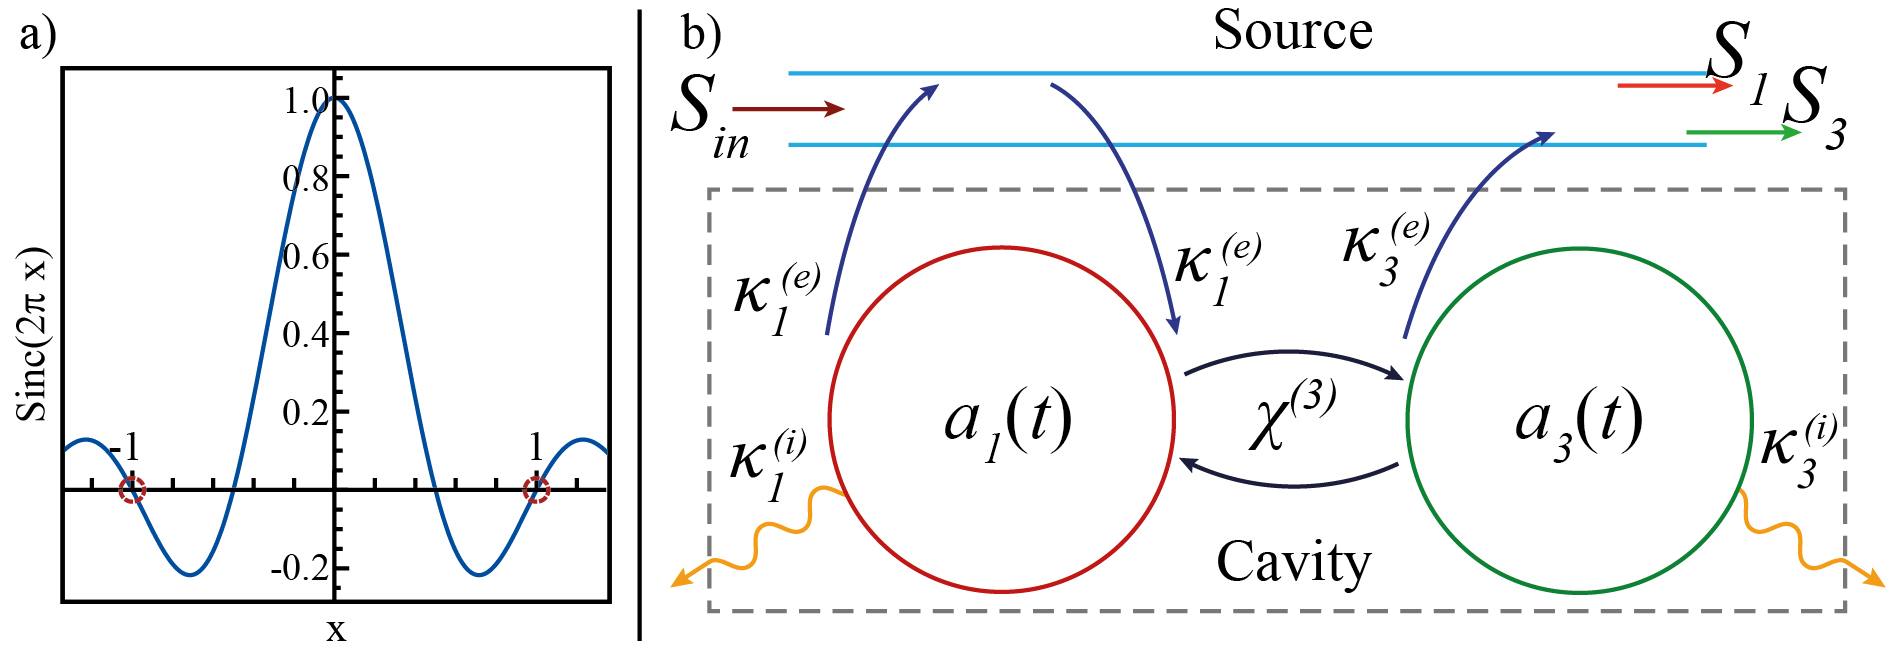
\includegraphics[width=16cm]{Dissertation_coupled_mode.jpg}
    \caption{\textbf{a) Sinc function:} The Sinc function of $2\pi x$ goes to zero for any integer $x$, but for $x=0$. \textbf{b) Lumped Model:} Our system are compound by a Cavity with two modes, both couple with bus waveguide that carry the input wave. The intrinsic loss and couple loss are different for each mode. The coupling between the modes occurs due to third order nonlinearity. }
    \label{fig:toy_model}
\end{figure}

\section{Numerical Results}

We will solve the Coupled Rate Equation using numerical methods. Our problem can be modeled as show in Fig~\subref{fig:toy_model}{b}. A system compound by a cavity with two modes, one in infrared ($a_1$) and one in visible ($a_3$), a input wave ($S_{in}$) with frequency near of the infrared mode. Both modes couple with the same bus waveguide that carries the input wave. The output waves are defined as 
\begin{subequations}
    \begin{align}
        S_1 &= S_{in} - \sqrt{\kappa^{(e)}_1}a_1\\
        S_3 &= \sqrt{\kappa^{(e)}_3}a_3
        \label{eq:out_wave}
    \end{align}
\end{subequations}

Initially, lest solve the Eq~\ref{eq:rate_broad} assuming a initial phase matching between the modes, that is, lets consider $\omega_3 = 3\times\omega_1$. The Fig~\subref{fig:temporal_solution}{a}
brings a well know bistable curve for the infrared mode (Red) while the Fig~\subref{fig:temporal_solution}{b} 
shows a slightly deformed lorentzian curve for the visible mode. This curve shape are true just if we assume that $\omega_3 = 3\times\omega_1$, which is not true due to the dispersion of the modes. A more general model assume that $\omega_3 = 3\times\omega_1 + \delta\omega$, in such case, the shape of the curve can be totally changed in function of the value of $\delta\omega$, we call this term phase detuning (do not mistake with the Detuning $\Delta_\alpha$). The Fig~\subref{fig:temporal_solution}{c}
shows some case. 

\begin{figure}[!h]
    \centering
    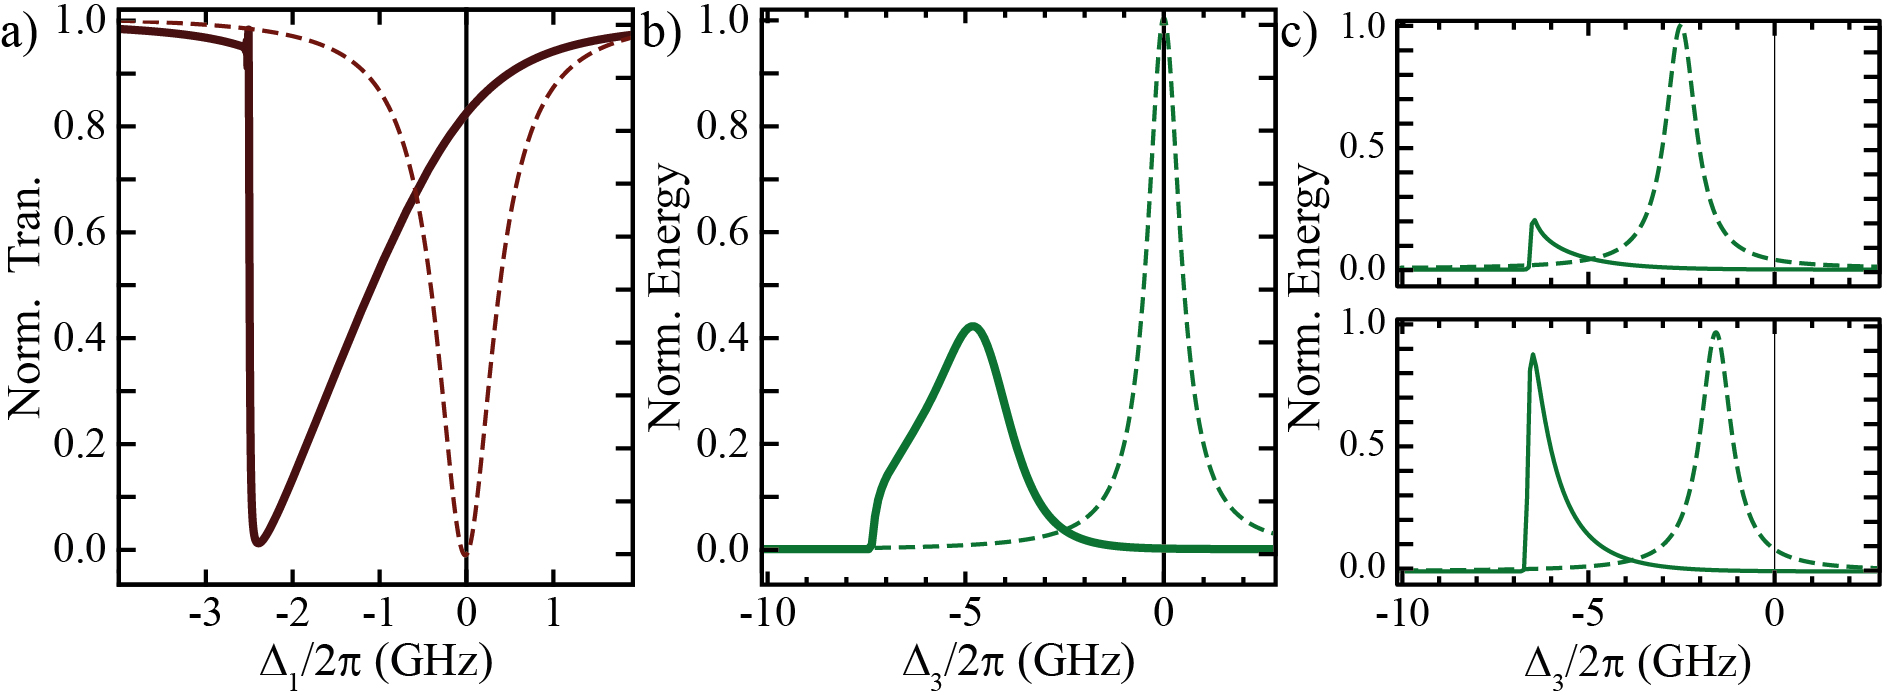
\includegraphics[width=16cm]{Dissertation_thg_solution.jpg}
    \caption{\textbf{Output in Function of the Detuning. a)} The solid line is the infrared transmission. The dashed line represents the initial state of the infrared mode. \textbf{b)} The solid line is the collected visible power (normalized by the optimal value). The dashed line represents the initial state of the visible mode. For this case, the phase detuning is zero. \textbf{c)} Results for different phase detuning. Upper $\delta\omega = 2\pi\times2.5$~GHz. Lower $\delta\omega = 2\pi\times1.5$~GHz, which is the close of the optimal case.}
    \label{fig:temporal_solution}
\end{figure}
This dynamics occurs due to the SPM and XPM terms. The displacement from the initial frequency are different for each mode which lead to different phase relation between the modes as long the source frequency is sweep. 

As we saw we Chapter~\ref{chap:optical_cavity} the displacement is direct related with the source power. A careful look to the solution for the Couple Rate Equation show that is always possible to find a situation, tuning both $\delta\omega$ and the power, that lead to a phase matching between the modes at the resonance. In this situation the conversion from the infrared to the visible are optimal. The phase detuning can be set by changing the temperature of the cavity. 

The refractive index of the material is a different function of the temperature for which frequency~\needcit, thus changing the temperature of the hole cavity will lead to a different displacement for the frequency infrared than for the visible. 

Let's assume now that for any input power we are able to find a temperature that lead the phase matching to occurs at the resonance. This assumption is similar to assume that the SPM, XPM and phase detuning are null in the Eq~\ref{eq:rate_broad}. The Fig~\subref{fig:power_solution}{a}
show the value of the ration between the collected visible power and the input power ($|S_3|^2/|S_{in}|$), which we define as Net Efficiency, in function of the input power. We are able to spot a critical power that lead to a maximum Third Harmonic Generation Net Efficiency. Moreover, this maximum is very stable in function of the power, the inset of Fig~\subref{fig:power_solution}{a} show that a variation of hundreds of Watts lead to a variation hundredth of the efficiency. For a specific scenario it is possible to reach a total conversion of photons from the infrared to the visible, the Fig~\subref{fig:power_solution}{b} shows the result considering this condition. 

\begin{figure}[h]
    \centering
    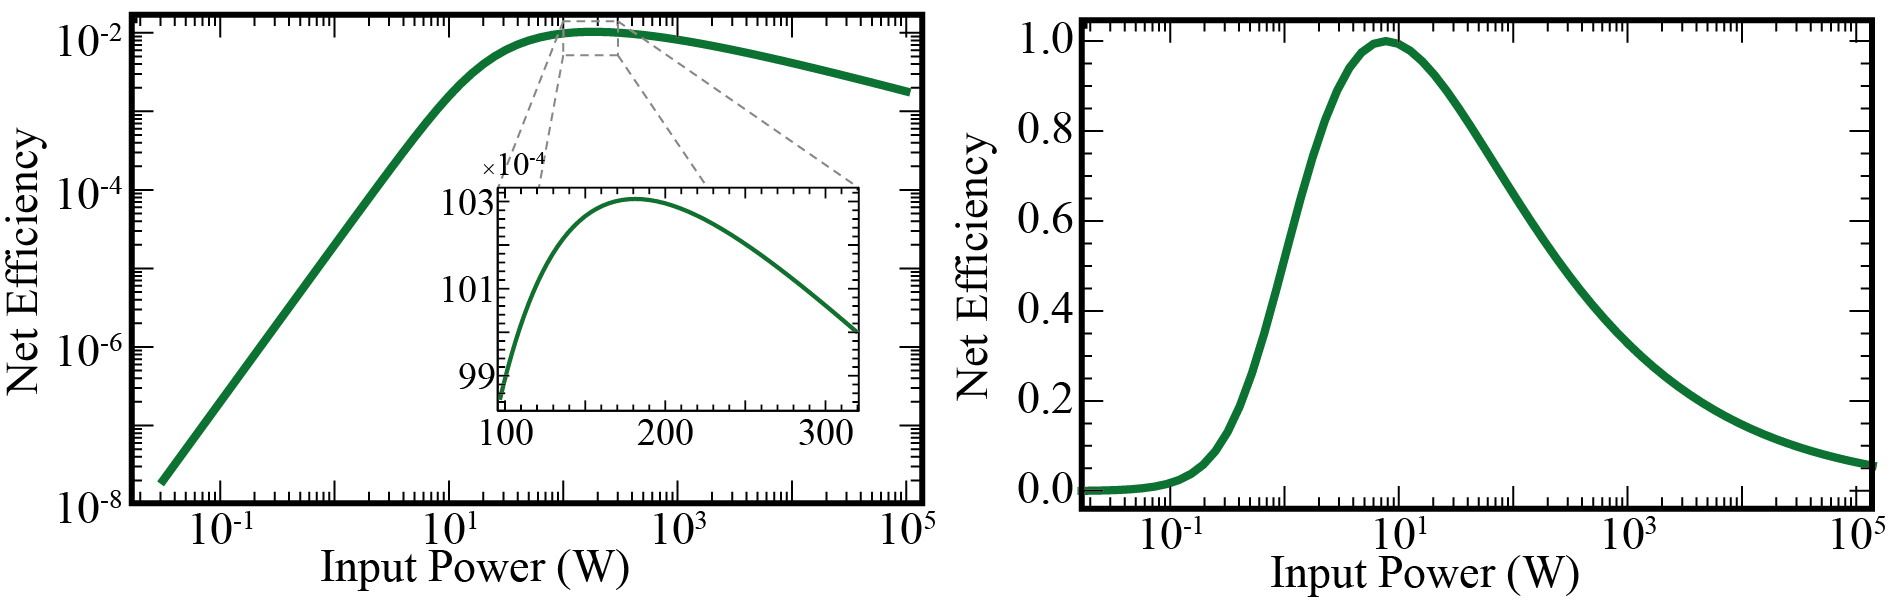
\includegraphics[width=16cm]{Dissertation_thg_eff.jpg}
    \caption{\textbf{Third Harmonic Generation Net Efficiency:} \textbf{a)} Numerical solution considering the values of the parameters close of the real system. \textbf{Inset:} Close look on the peak of efficiency. \textbf{b)} Numerical solution considering $\kappa^{(e)}/\kappa^{(i)} = 10^3$ for both, infrared and visible modes.}  
    \label{fig:power_solution}
\end{figure}

The most important assumption to reach a total conversion scenario is that the couple rate $\kappa^{(e)}$ must be much high than the loss rate $\kappa^{(i)}$ for both, infrared and visible, which lead to a engineer problem. Our coupling system, a tapered optical fiber, is optimized for the infrared mode, so the coupling with the visible mode is weak.

\section{Conclusion}

In this Chapter we have applied perturbation theory in order to develop a Rate Equation that couple two modes due to third order nonlinearity. This procedure lead us to few new terms, two phase modulation terms, self and cross (SPM and XPM), and the couple terms $B_1$ and $B_3$.

The overlap integral J3, Eq~\ref{eq:overlap_j3}, lead to the relation $m_3 = 3\times m_1$ for the coupled modes, which is necessary for phase matching. Meanwhile, the SPM and XPM displace differently each mode, leading to a phase detuning of the modes. Nevertheless, as the displacement is a function of both, PM terms and the power, is possible to set specific values of power and initially phase detuning that lead to a perfect phase matching in the resonance frequency. 

If we consider a situation where the system is always in phase matching, the solution of the Coupled Rate Equation show a critical power wheres the efficiency of Third Harmonic Generation is maximized. This maximum occurs in a large band of power.

In order to verify the validation of this theoretical results, we proposed some set of experiments. The following Chapter shall treat this subject.  